\section{Exercises of Chapter 2}

\begin{enumerate}

	\item {\bf Discuss the dichotomy of rocket science in the modern era.}\\
	
The first dichotomy starts after WWI, with the Treaty of Versailles that prohibited Germany to develop long-range artillery and the NAZI Germany developed the V2 (\textit{Vergeltungswaffe 2}), that was a missile capable of reaching an objective 300 km away from the launch place. The ''success'' of this lethal weapon, led the governments of the Soviet Union and USA to start developing their own missiles.

The second dichotomy happens when the Soviets where the firsts to place a satellite in orbit (Sputnik), and with this, the space era started. The objective of building rockets was not anymore only military, but it was also scientific and even commercial. 

	\item {\bf In your own words give a definition for a rocket mission.}\\
	
A mission is the objective that the government of a country or a private organization has for which a rocket is needed to be accomplished. Examples are; putting a satellite in GEO, sending a robot to Mars to make experiments, sending a missile with an atomic bomb to an asteroid that is going to impact our beautiful home planet.
	
	\item {\bf What is a payload?}\\
	
The payload is the equipment that solves the problem represented by the mission. In other words, the payload is how the mission is intended to be accomplished.

For the mission \lq\lq{}putting a satellite in GEO\rq\rq{}, the payload is the satellite.\\
For the mission \lq\lq{}sending a robot to Mars to make experiments\rq\rq{}, the payload is the robot.\\
For the mission \lq\lq{}sending a missile with an atomic bomb to an asteroid that is going to impact our beautiful home planet\rq\rq{}, the payload is the bomb.

The payload is the all hardware above the launch vehicle, except the protective fairing, which is also part of the launch vehicle. 
	
	\item {\bf What is the so-called “SMAD”?}\\
	
SMAD stands for \textit{Space Mission Analysis and Preparation}, and it is the name of book, that according to \cite{book}, is the standard text book for space mission preparation.
	
	\item {\bf Give the four basic assumptions required for understanding the basics of projectile motion.}\\
	
\begin{enumerate}
1. Acceleration due to gravity is constant\\
2. No air resistance\\
3. Earth is flat\\
4. Earth’s rotation has no impact on the motion of the projectile.
\end{enumerate}
	
	\item {\bf Define MECO.}\\
	
MECO stands for main engine cutoff, and it happens when the main engine is turned off, it can be because all the propellant has been used, or also in a multistage rocket it can be that the first stage that contains the main engine still has propellant which is going to be used for the landing of the first stage.
	
	\item {\bf Equation 2.9 gives the parabolic flight path of a rocket trajectory as height, \textit{y}, as a function of range, \textit{x}, or \textit{y(x)}. Use the quadratic equation to solve for \textit{x} as a function of \textit{y} to give a range equation as a function of height.}\\

\begin{equation} \label{eq:x_of_y}
	x(y-y_{bo})  = \frac{v_{bo}^2 \cos\theta}{g}(\sin\theta \pm \sqrt{\sin^2\theta-\frac{2g(y-y_{bo})}{v_{bo}^2}})+ x_{bo} 
\end{equation}

Figure \ref{fig:exercise7} shows \textit{x(y)}.
	
\begin{figure}[H]
	\centering
	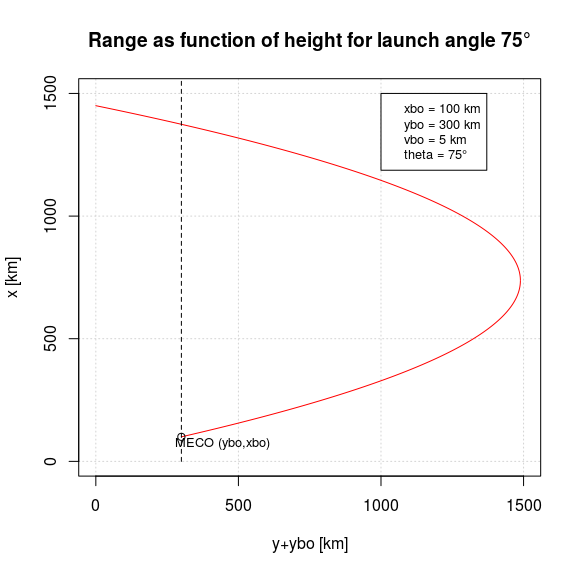
\includegraphics[width=0.7\textwidth]{exercise7.png}
	\caption{Range as a function of height \textit{x(y)}.}
	\label{fig:exercise7}
\end{figure}	
	
	\item {\bf A rocket is launched with a burnout velocity of 75 m/sec, burnout altitude of 300 m, and a burnout range of 100 m. Assuming a flight path angle of 75\degree, calculate the final range of the rocket when it impacts the ground.}\\

Substituting values into eq. 2.14 from the book. \\

\begin{equation}
	x_{max}  = x_{bo} + (v_{bo}\cos\theta)\left[ \frac{v_{bo}\sin\theta+\sqrt{v_{bo}^2\sin^2\theta+2gy_{bo}}}{g}\right]
\end{equation}

\begin{equation}
	x_{max}  =  100 + (75\cos75\degree)\left[ \frac{75\sin75\degree+\sqrt{75^2\sin^2(75\degree)+2(9.81)(300)}}{9.81}\right] = 452.1426 [m] 
\end{equation}

This value can also be observed in figure \ref{fig:exercises_8_9_10}.
	
	\item {\bf Calculate the maximum altitude reached by the rocket in Exercise 8.}\\
	
Substituting values into eq. 2.11 from the book. \\

\begin{equation}
	y_{max}  =  y_{bo} + \frac{v_{bo}^2 \sin^2\theta}{2g}
\end{equation}

\begin{equation}
	y_{max}  =  300 + \frac{75^2 \sin^2 75\degree}{2(9.81)} = 567.49 [m]
\end{equation}	

This value can also be observed in figure \ref{fig:exercises_8_9_10}.

	\item {\bf Redo Exercise 8 to determine the range at MECO altitude. What is the range at MECO if the initial flight path angle is 15\degree ?}\\
	
As explained in the book, the range at MECO for two angles whose addition equals 90\degree (75\degree + 15\degree = 90 \degree), the range at MECO is the same. Substituting values into equation \ref{eq:x_of_y} the range at MECO for 75\degree and 15\degree can be obtained.

\begin{equation}
	x(y_{MECO}-300)  = \frac{75^2 \cos15\degree}{9.81}(\sin15\degree + \sqrt{\sin^2 15\degree -\frac{2(9.81)(300-300)}{75^2}})+ 100 = 386.697 [m]
\end{equation}	
	
\begin{figure}[H]
	\centering
	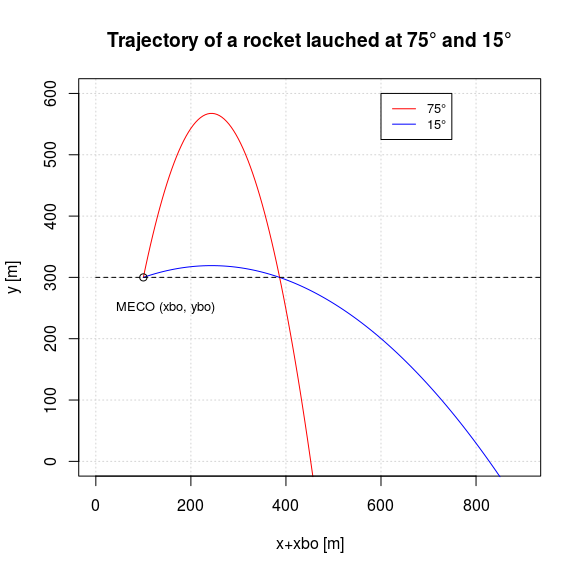
\includegraphics[width=0.7\textwidth]{exercises_8_9_10.png}
	\caption{Trajectory of rocket launched at 75\degree and 15\degree .}
	\label{fig:exercises_8_9_10}
\end{figure}

	\item {\bf What is the force due to gravitational attraction between the Earth and the Moon? Assume the Moon is 400,00 km from Earth and the mass of the Earth is $5.99 x 10^{24}$ kg, and the mass of the Moon is $7.36 x 10^{22}$ kg.} 	

	\item {\bf  A satellite is in a circular orbit at 100 km above the Earth. What is the orbital velocity of the satellite? How long does it take for the satellite to make one complete orbit around the Earth?} \\
	
	\item {\bf What is the semilatus rectum?} \\
	
	\item {\bf  Give the equation for a conic section.} \\
	
	\item {\bf  A spacecraft is traveling in an orbit with periapsis at 100 km and apoapsis at 1000 km. What is the eccentricity of the orbit? This orbit is what type of conic section?} \\
	
	\item {\bf Calculate the semilatus rectum of the spacecraft orbit in Exercise 15.} \\
	
	\item {\bf What is the period of the orbit described in Exercise 15?} \\
	
	\item {\bf What is the velocity of the spacecraft in Exercise 15?} \\
	
	\item {\bf Calculate the  $\Delta v$ needed to circularize an elliptical orbit with an apoapsis at 500 km above the Earth and a periapsis at 325 km above the Earth. (Hint: see Example 2.3.)} \\
	
	\item {\bf Calculate the $\Delta v$ burns needed to conduct a Hohmann transfer from a 300 km circular orbit around Earth to a 35,000 km circular orbit around Earth.} \\	
	
	\item {\bf Calculate the transfer time for the Hohmann transfer given in Exercise 20.} \\	

	\item {\bf A Space Shuttle is in a 325 km circular orbit in a 28\degree inclination. How much $\Delta v$ is needed to move the Shuttle to a 51\degree inclination?} \\	

	\item {\bf What is $C_3$} \\	

	\item {\bf A Mars probe leaves Earth’s sphere of influence with a $C_3$ of 16 $km^2/sec^2$. How much $\Delta v$ is required for the probe to enter a Mars orbit
with periapsis at 100 km and apoapsis at 1,000 km?} \\	

	\item {\bf In order to go from Equation 2.87 to Equation 2.88 (as well as Equation 2.89 and Equation 2.90) some algebra was needed. Do the algebra calculation showing all the steps.} \\	

	\item {\bf A ballistic missile has a powered flight range angle of 4\degree and a reentry range angle of 5\degree. If the missile has a total ground range of 8,000 km, what is its free-flight range angle? (Hint: Assume the 8,000 km range is the distance the missile travels around the circumference of the Earth. The radius of the Earth is 6,370 km.)} \\	
	
\end{enumerate}


























